\chapter{Concepts and Architecture}

\section{Prerequisite}
As describet in the chapter Secure Scuttlebutt we have an ID centric single feed driven environement. This prerequisite changes from the beginning. Central idea of the Feed Bundling Protocol is to split up this ID centric environement into replicated feed pairs, where two participants hold at least one of such a pair. This pair contains the whole dialog between two nodes which have a contract together.\\
Look at it as a tin can phone from your childhood where you have two cans, strapped together for every friend you want to communicate with. You start with one corded phone to your best friend, the one you trust the most. In one you talk and the can 'saves' everything you say to it. on the other side your friend has the same but can only hear things out of one can and can only talk into the other. Having this, the dialog needs a way or language to express expectations or requests from either side to communicate with each other, where you can declare what you want from each other. After quiet some time it will eventually get boring only talking to this one friend. Luckily your friend is the coolest kid in school and knows everyone and even tells you who he knows. So you decide tho ask your friend if he could introduce you to his other friends. Having that we got the introduce mechanic which adapts exactly this social human behaviour. After your friend has introduced you to one of his friends you and your friend start to build the new tin can phone. But because you are too far away from each other you cannot just have a cord from one to the other. So your best friend is ready as always and helps you by passing to cord trough his house. This corresponds to the replication of the feeds over intermediary connectivity provider. Yet another problem occures, you are not the only one. after quiet some time your bestfriend has so many strings in his house from al his friends which want to talk to that other friend. he repeats all the phones there so he has an enourmous amount of strings going to that other friend. SO he decides to combine all these strings into one and send all messages trough this single one with the information into which can it should come at the end. He multiplexes. Given that little story we can derive concepts and architecture for the tin can phones of the future.
\section{Contracts}
Deriving from that little story we see the base in the friendship. the friendship between you and your best friend and the friend ship between your bestriend and his other friend. So first and foremost of the whole connectivity, protocol and bundling, lay the business contracts between the nodes. Throughout the whole process of the these contracts and relationships between each participant got questioned and modified, since this is the most important aspect or basic building block for the whole thesis.\\

\subsection{Client-ISP Contract}

To build the tin can phone three basic identifiers are needed. First of all you have to trust each other. This accords to the whole juristical contract between the to parties. Next you need to know your names to lable the phone, so you know to who you talk. This refers to the public keys. Since everybody in your house can use the tin phone you also need some sort of secret so your friend know you send the message not your mom. This refers to the private key. Having that you need your two tin cans and two wires. One can stands for one feed and the wire for the replication. But if you do not know the address of your mate you do not know where to put that wire, hence you need that too. The address, as the name is well chosen, refers to the IP-address. To keep things a little easier we perform everything on a localhost in the file system so the address corresponds to a path or location to or of a folder. Last but not least, to distinguish all the cans you lable them accordingly. This leads to a contract like that.\\



\begin{tabular}{llll} \toprule
    Client-Contract&value&ISP-contract&value\\ \midrule
    actual public key:& cli001 &  actual public key: &isp001  \\ 
    actual private key:& ****** & actual private key:& ****** \\
    actual feed ID:& cli001\_isp001 &actual feed ID:&isp001\_cli001 \\ 
    ISP public key&isp001&Client public key:&cli001\\
    ISP feed ID&isp001\_cli001&Client feed ID:&cli001\_isp001\\
    ISP location:&.\slash isp001\slash &Client location:& .\slash cli001\slash \\\bottomrule
\end{tabular}
\subsection{ISP-Server Contract}
Since your best friend has an other friend the contract is the same as in the Client-ISP Contract.\\\\
\begin{tabular}{llllll} \toprule
    ISP-contract&value&Server-Contract&value\\ \midrule
    actual public key:& isp001 &  actual public key: &ser001   \\ 
    actual private key:& ****** & actual private key:& ******  \\
    actual feed ID:& isp001\_ser001 &actual feed ID:&ser001\_isp001\\ 
    Server public key:&ser001&ISP public key:&isp001\\
    Server feed ID:&ser001\_isp001&ISP feed ID:&isp001\_ser001\\\bottomrule
\end{tabular}
\\\\
Clearly seen, that client and server are indirectly 'connected' over isp001, which refers to your best friend. Initial idea of the thesis was a peer to peer Internet Connectivity Provider (ICP) network where the ISP-Company distributes the feeds internally between the ICPs. So in real life there is a contract the ISP e.g. Swisscom and the keys refer to connectivity provider stations or nodes within the ISP newtork of ICPs. Which means cli001 has a connection with icp342 and server has a contract with icp903. But both have a contract with Swisscom, which has internal routing to pass information from icp342 to icp903 - but more in the Outlook section.
\\
\begin{figure}
    \centering
    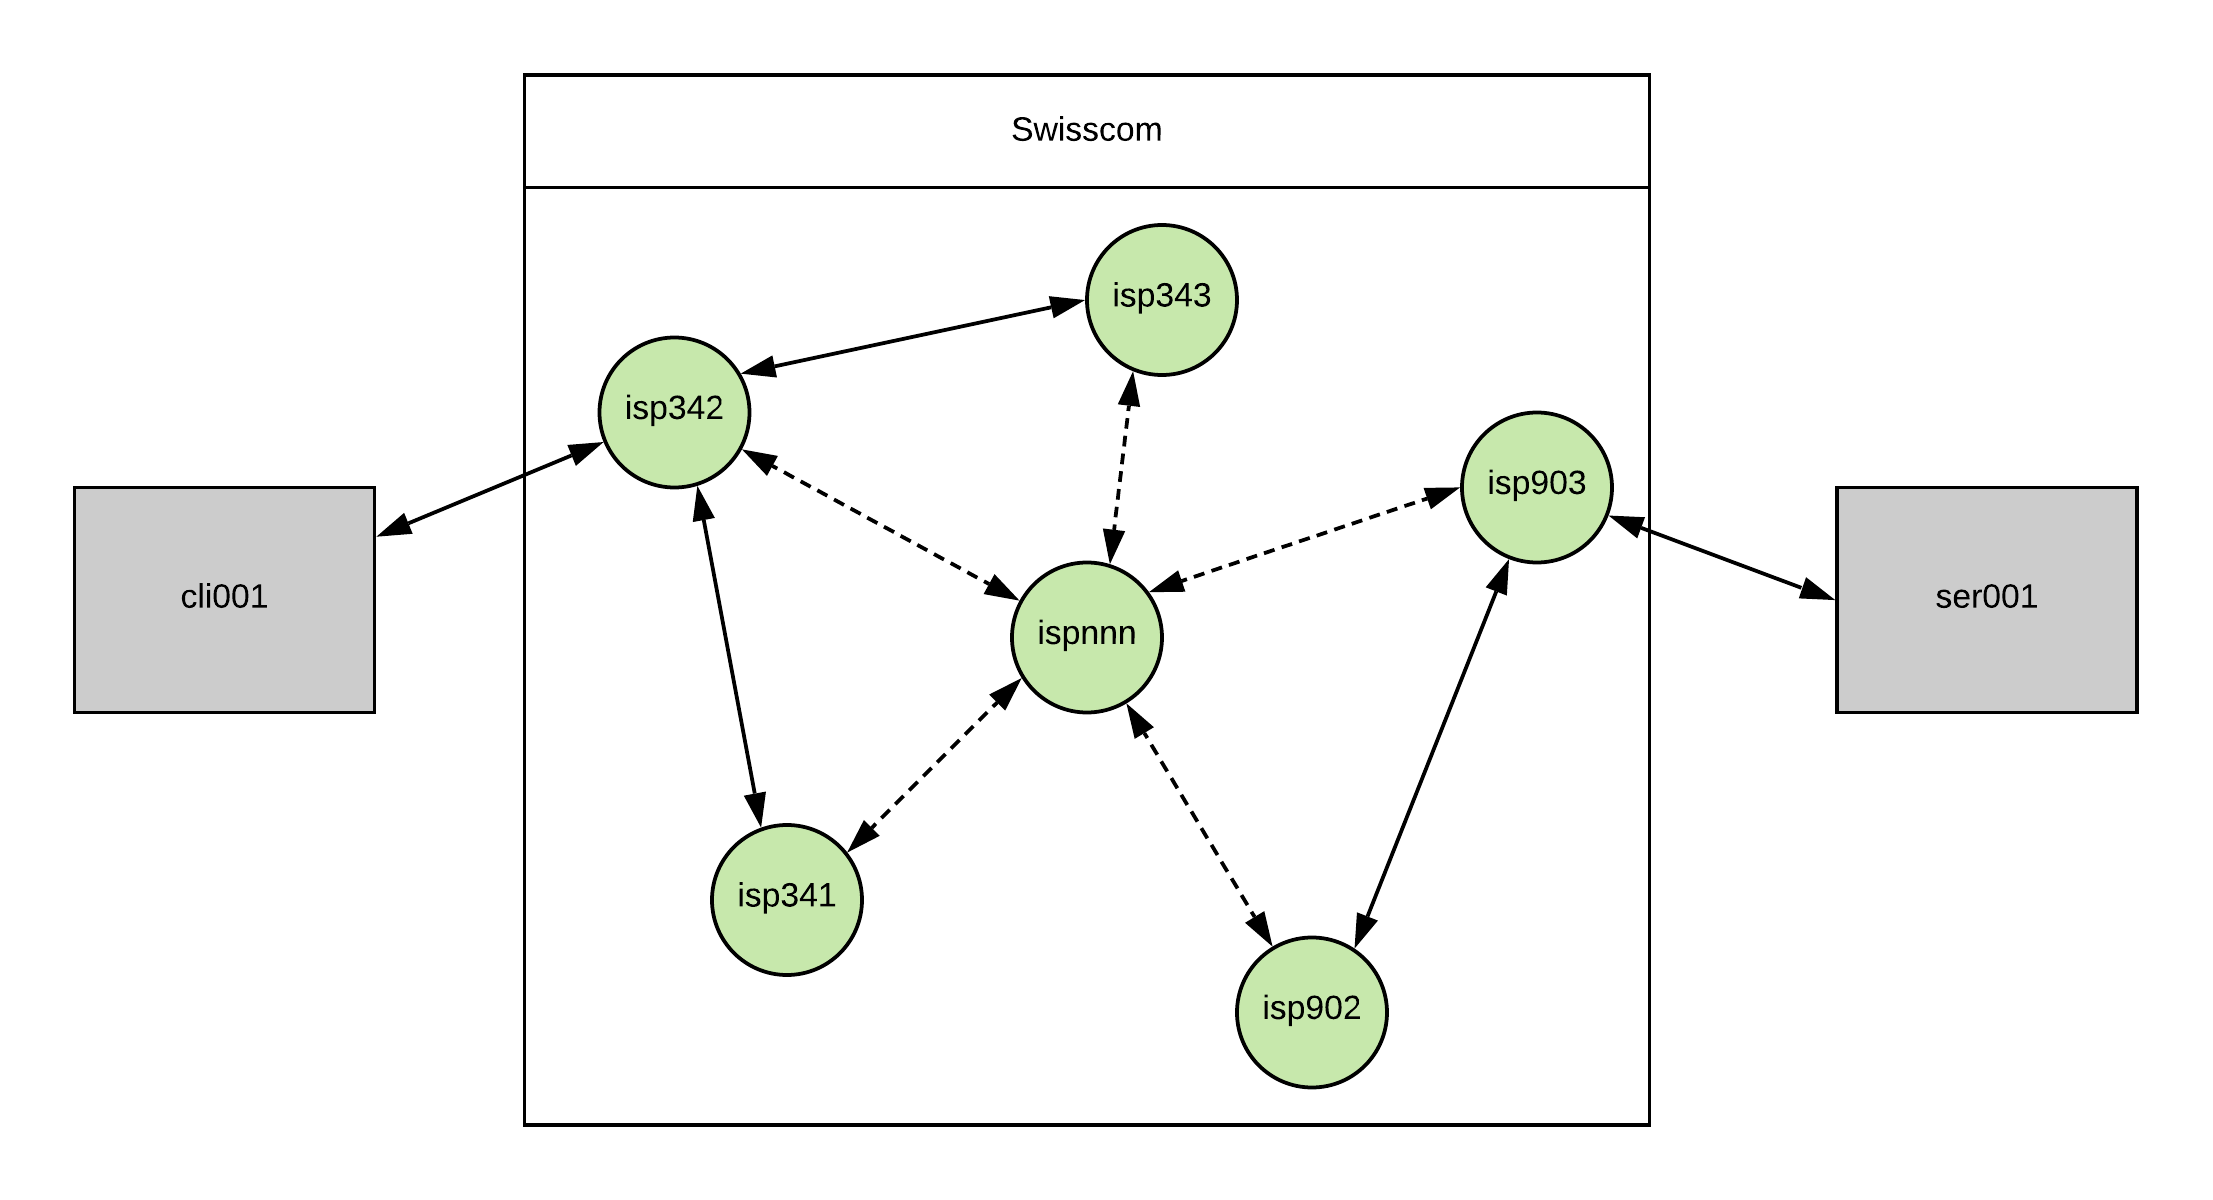
\includegraphics[width=0.9\textwidth]{p2p_contracts}
    \caption{A simplified contract network.}
    \label{fig:contract_network}
\end{figure}



Since now a contract is established, we need to know what happens in the tin cans and the wire. This leads to the replicated feeds.

\pagebreak

\section{Replicated Feeds}
From the SSB API the following sentence can be exctracted: "A feed is a signed append-only sequence of messages. Each identity has exactly one feed.\footnote{\url{https://scuttlebot.io/more/protocols/secure-scuttlebutt.html}}"
So what do these properties mean?
\begin{itemize}
    \item signed message: Signing a message means the encryption of plain text with the sender's private key to a cipher text. The crypto text can be deciphered with the sender's public key.
    \item append-only: Under append-only we understand that this sequence can not be forged. So there is no possible way to modify or delete any entries that were appended at any time\footnote{Feeds - \url{https://ssbc.github.io/scuttlebutt-protocol-guide/}}. This append-only property is realzied with a hash chain which referenzes the hash value of the perviously generated message.\footnote{Feeds - \url{https://ssbc.github.io/scuttlebutt-protocol-guide/}}
    \item identity - one feed: Meant here is the perviously mentioned ID centric architecture. Per identity (key) is only a single feed mapped, where every, and I mean every, information you created or used in the SSB universe is stored.
\end{itemize}
Simplified a schema can be pictured, in the SSB feed is much going on but an adapted simplified version is more than sufficient for this thesis.

\begin{figure}
    \centering
    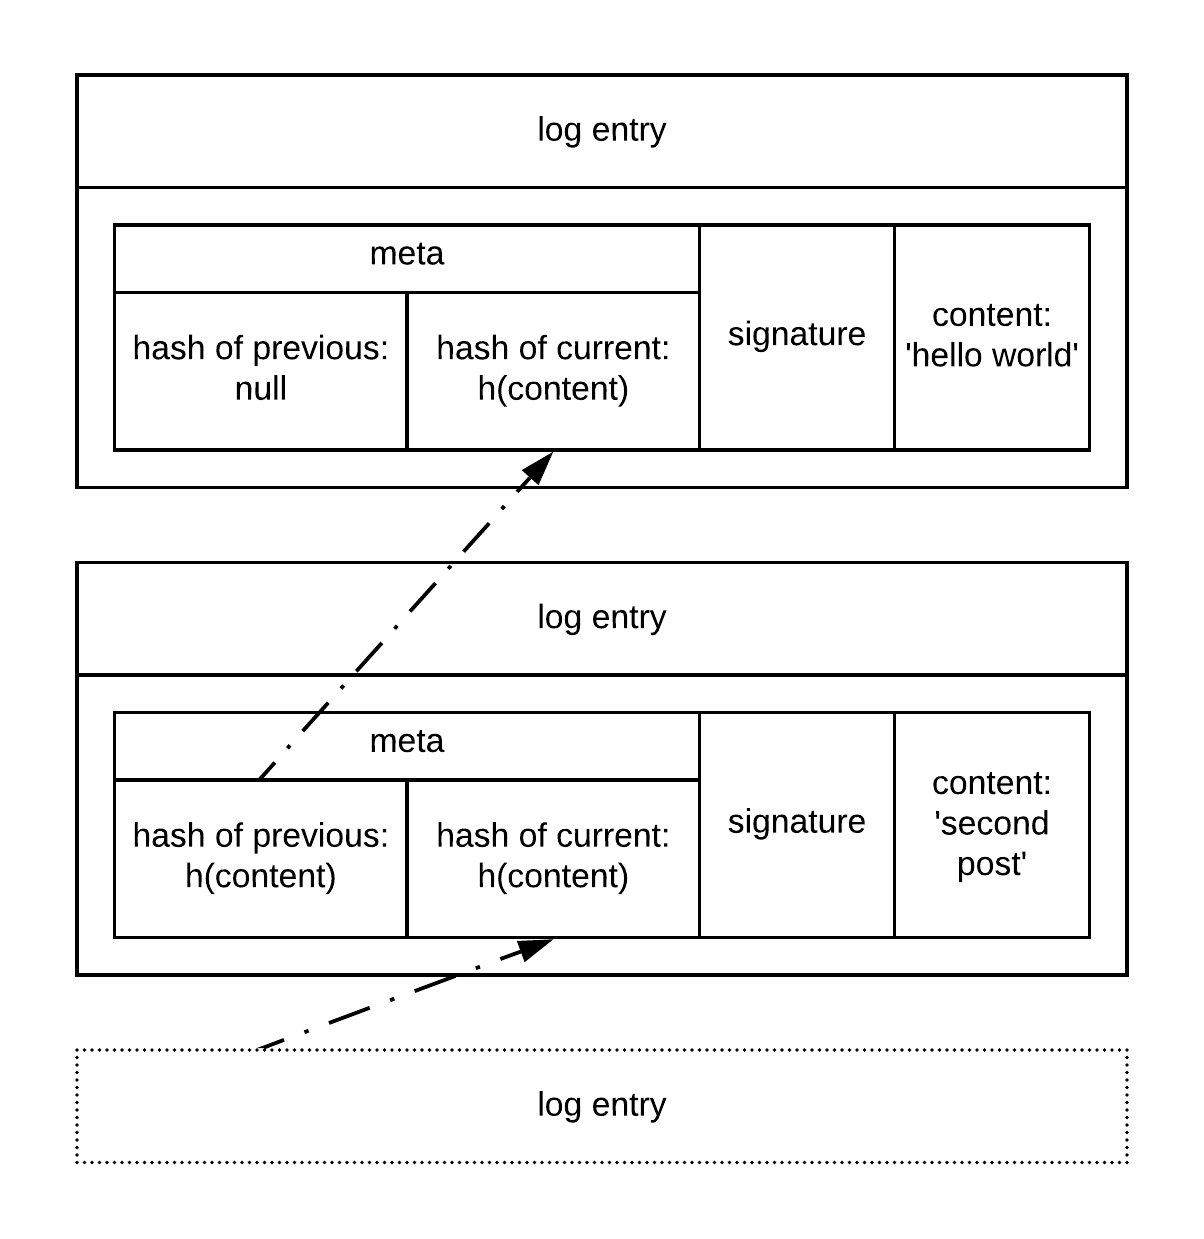
\includegraphics[width=0.5\textwidth]{feed_schema}
    \caption{A schematic simplified feed.}
    \label{fig:feed_schema}
\end{figure}

So what can be derived from these information? Signing ensures that you can trust an identity. The append-only property underlines this trust by guaranteeing completness of the information read in a feed. ID centric feeds ensure that this feed belongs to exactly one identity but there is the sticking point. Since the replication of the SSB protocol always replicate the whole feed to all peers (hops noch angeben) of a single identity there is a massive load on the wire for big feeds. This causes latency and long scuttling time (feed update). \\
By splitting the feeds into smaller feeds this can be bypassed and the effective communication between two parties bundled in the already mentioned feed pairs. Resulting we have a schema like this:
\begin{figure}
    \centering
    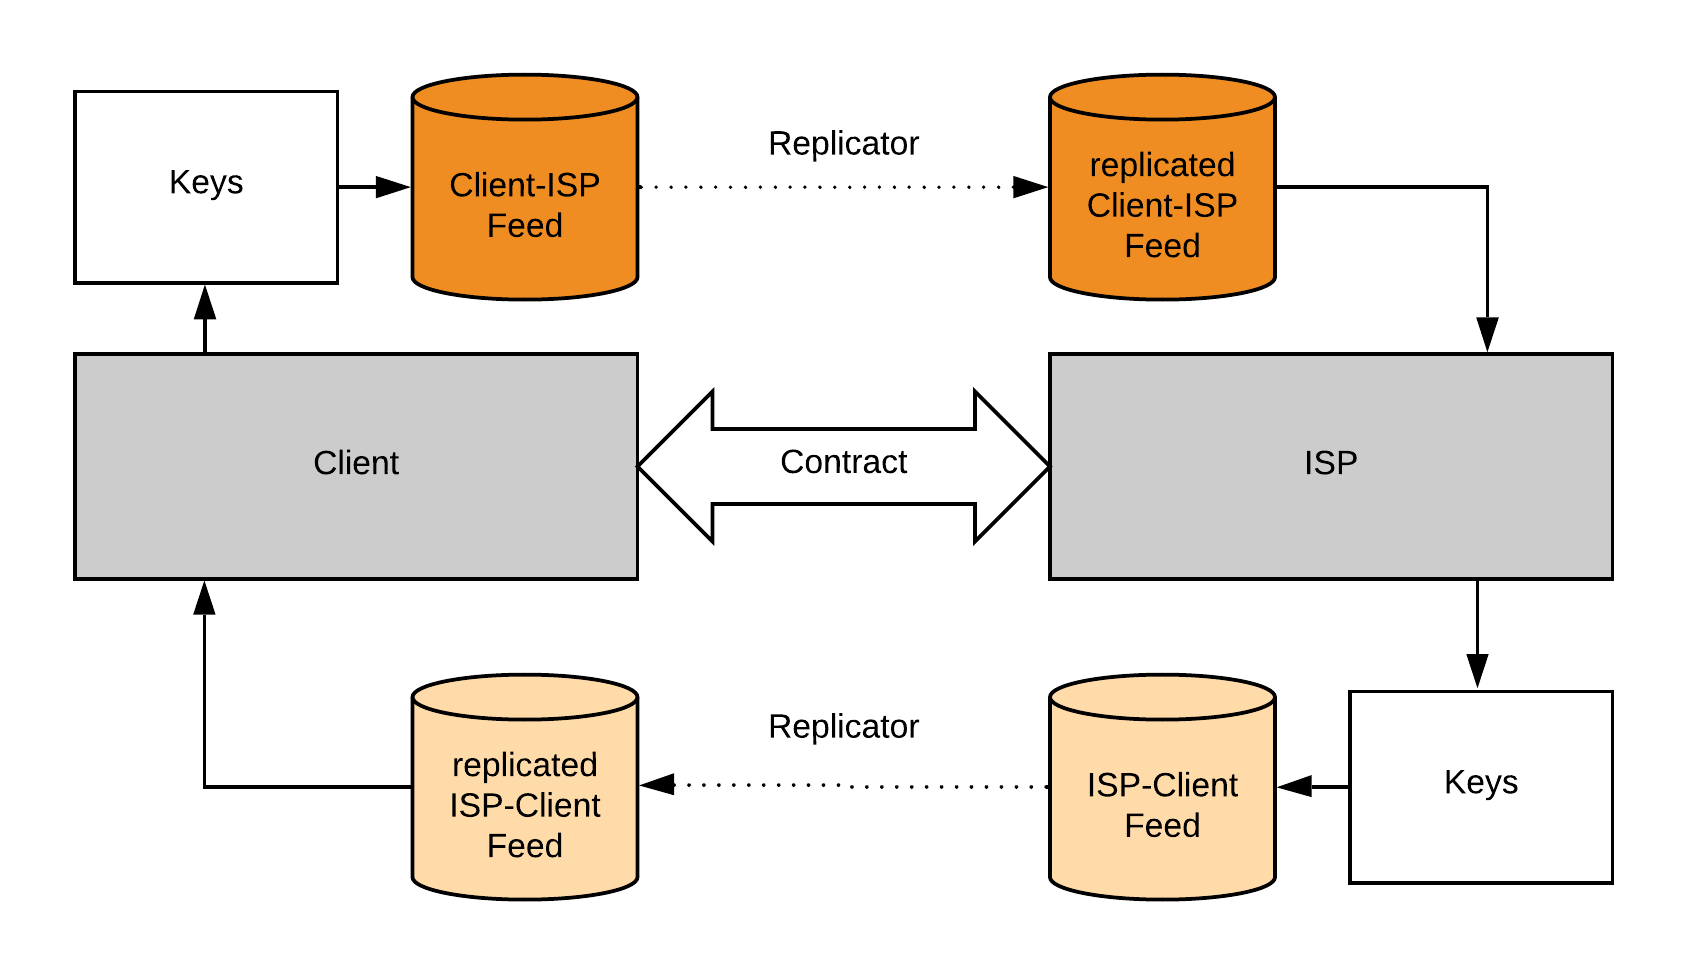
\includegraphics[width=0.9\textwidth]{fbp_v0_1_Schema}
    \caption{Full contract between client and ISP with feeds.}
    \label{fig:contract_cli_isp}
\end{figure}
For the skae of clarity only the situation between client and ISP is given. since for server and isp it is the same. As you can see. The replicator or the replication process has it first apperance. As concept, there is some sort of replicator instance or procedure that replicates the feeds to the corresponding address or location. We have a closer look in the implementation.\\

Having this setup the next step is to have a possibility to communicate, so the client can request information from the isps real database

\pagebreak
\section{Remote Procedure Call}
General explanaiton of RPC.

\subsection{Send Request}
Format of request and api of method
\subsection{Read Request}
Format of request and api of method
\subsection{Send Result}
Format of request and api of method
\subsection{Read Result}
Format of request and api of method

Resulting schema of the API and descriptions given above:

\begin{figure}
    \centering
    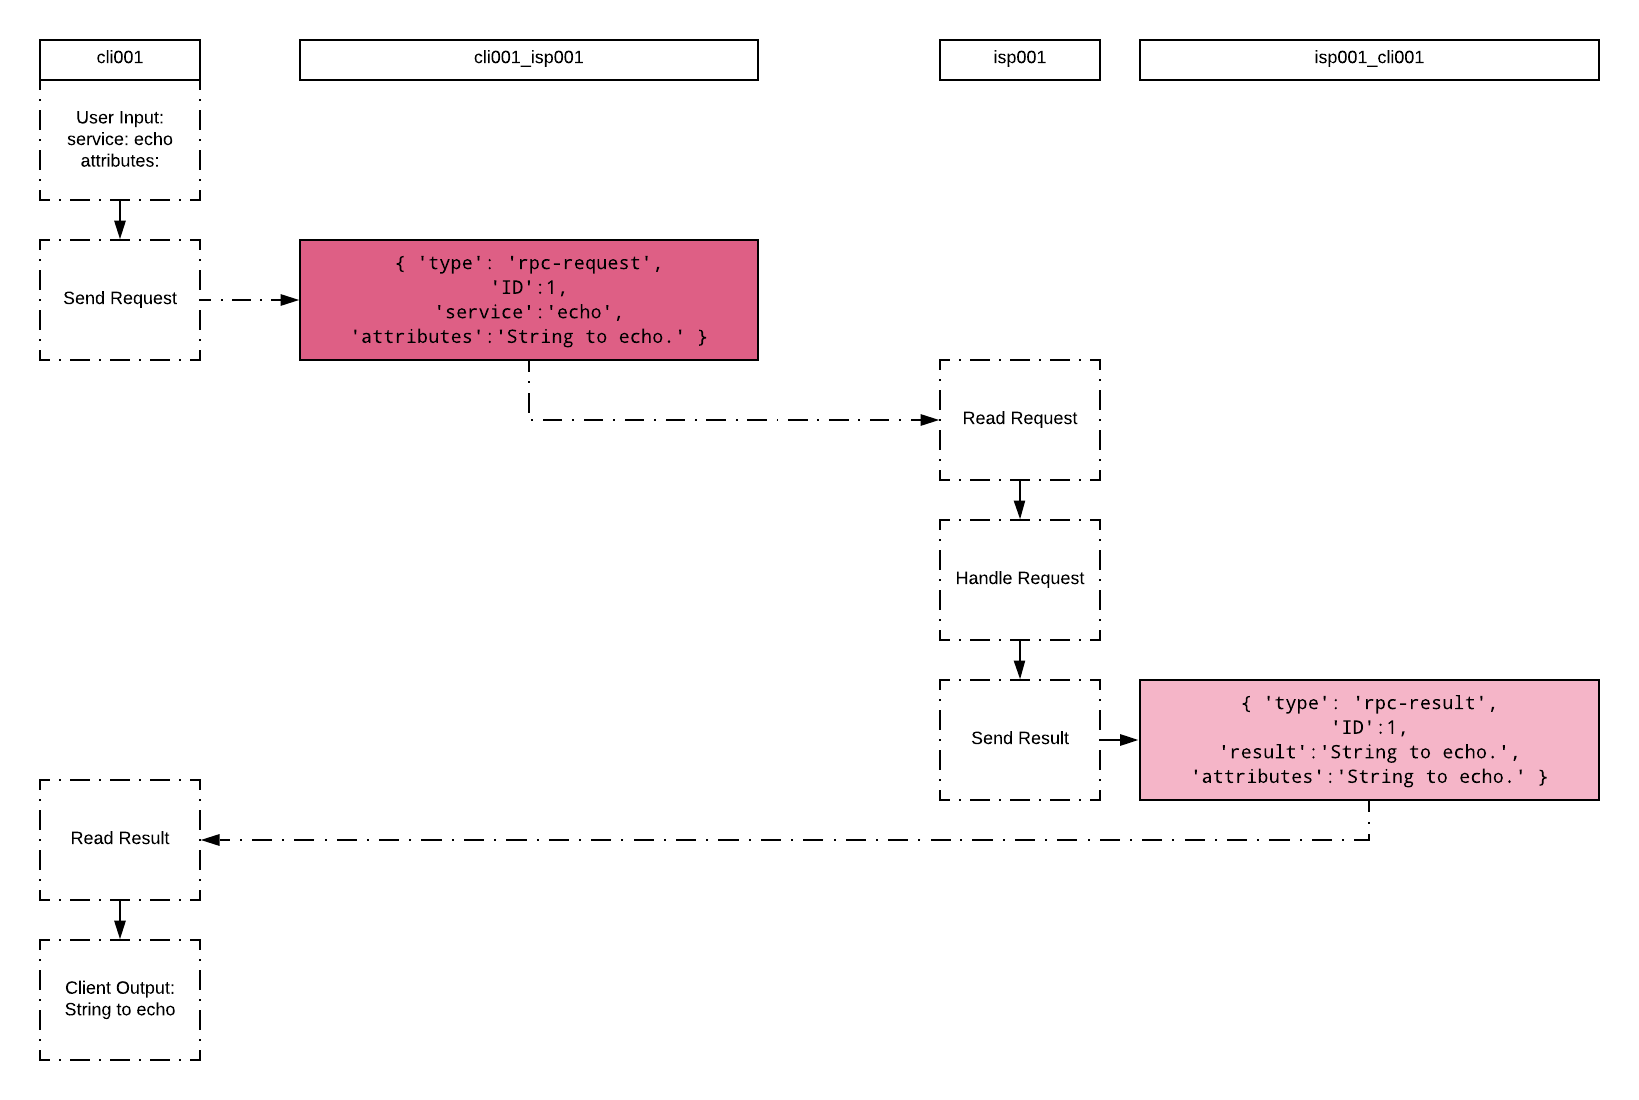
\includegraphics[width=0.9\textwidth]{rpc}
    \caption{A Remote Procedure Call by cli001 to isp001.}
    \label{fig:contract_cli_isp}
\end{figure}


Picture description: -> will be splited into above sections

Seen in the picture above, client cli001 makes a request of the echo service with the attribute: String to echo. This is passed to the send\_request function which assigns an unique ID for this request, resulting from the already given ids in the feed pair. Also merges type, id, service, and attributes into a request (a defined datastructure), writes appends this as a new log entry to the feed and saves the ID for keeping track of open requests. isp001 now detects a change on the feed cli001\_isp001 and invokes the read\_request method which takes the request appart and evaluates the service. Now the request gets handled and the wanted value returned. After that send result is invoked. It is similar to the send request, difference is the type and the result is also appended to the result datastructure. Now again, writing a new log entry to the feed with the given content. cli001 is notified that the isp001\_cli001 feed is changed. so read result is invoked and the result gets either to the program, where it was requested or printed to the client.

%\section{v0.2}
%The next step was to include servers with services. Also here the Prerequisite and contract situation changed.
\section{Introducing and Detrucing}
\subsection{Introducing}
Recaping the tin can phone story: The idea of introducing is to get in contact with a new friend, where your bestfriend introduces you to him. You and your new friend handcraft a new tin can phone. Since the cord only is as long as it reaches your bestfriend, he connects you to your newly aquired friend. \\

So the general idea of introducing in context of the feed bundling protocol is onboarding to a new server over your ISP. This approach differs from the commonly spread pubublish and subscribe (pub/sub) architecture. Whereas the server has no choice to decline a client in the pub sub model this is a foundation of the introduce detruce model. More technical
General Idea - 
onboarding to a server. Instead of following server - introduce to server. differs from pub sub pattern in the way that the server has the choice to accept or decline a client. As we were talking of rpc before, in either way accept or decline an answer is provided to the client, else it would violate the rpc clauses.

So lets tank about the procedure in more detailed way: cli001 sends a rpc request to the introduce service of his ISP. this request needs an attribute which specifies the server the client wants to be intrduced to. In this particualr case ser001.
isp001 invokes the introduce service, which now makes rpc request with information about client and the fact, that it wants to introduce itself to ser001. and sends this to the server. Now the server has the coice to either accept or decline the introduce inquiry. If ser001 accepts the introduce it will directly create the feed pair on his side (the two tin cans). afterwards it sends a confirmation or acceptance back to the ISP. Additionally to just the statement that the client was accepted the whole contract information for client is given by server: feed ID etc. 
Or the server declines the introducing approach, so the result is rejection followed by no or some sort of empty contract.

Either way isp001 gets the result and passes this result to the initial rpc request from the client. The client now gets his result. According to the state of acceptance or rejection it builds his feed pair in accordance with contract. finally the connection is established. Now if client wants to use a service from server it only writes the request in the corresponding feed and the procedure is the same as described in RPC Section.
\\
An important addition, only client can introduce itself. The server has no knowledge about clients and also no way to get knowledge about clients, so only client can ask server for a contract. 

\subsection{Detrucing}
Detrucing as a newly invented word by me, since normally after you introduced yourself to a person there is no way to make this unhappened. It acts the same for unfollow in a pub sub domain. But in contrary to the introduce both parts of the contract can detruce. \\
precisely either client or server can send a rpc request to the ISP service detruce which gets propagated to the opponent descibed above in the introducing part and results in terminating the whole contract. Result of this action is deleting keys and feeds. There is no way to decline a detruce service request.
\\
Also here an important addition, after detrucing from either side, the client can yet again introduce itself to server.
\\
Taken these descriptions a new schema of the network derives.
\begin{figure}
    \centering
    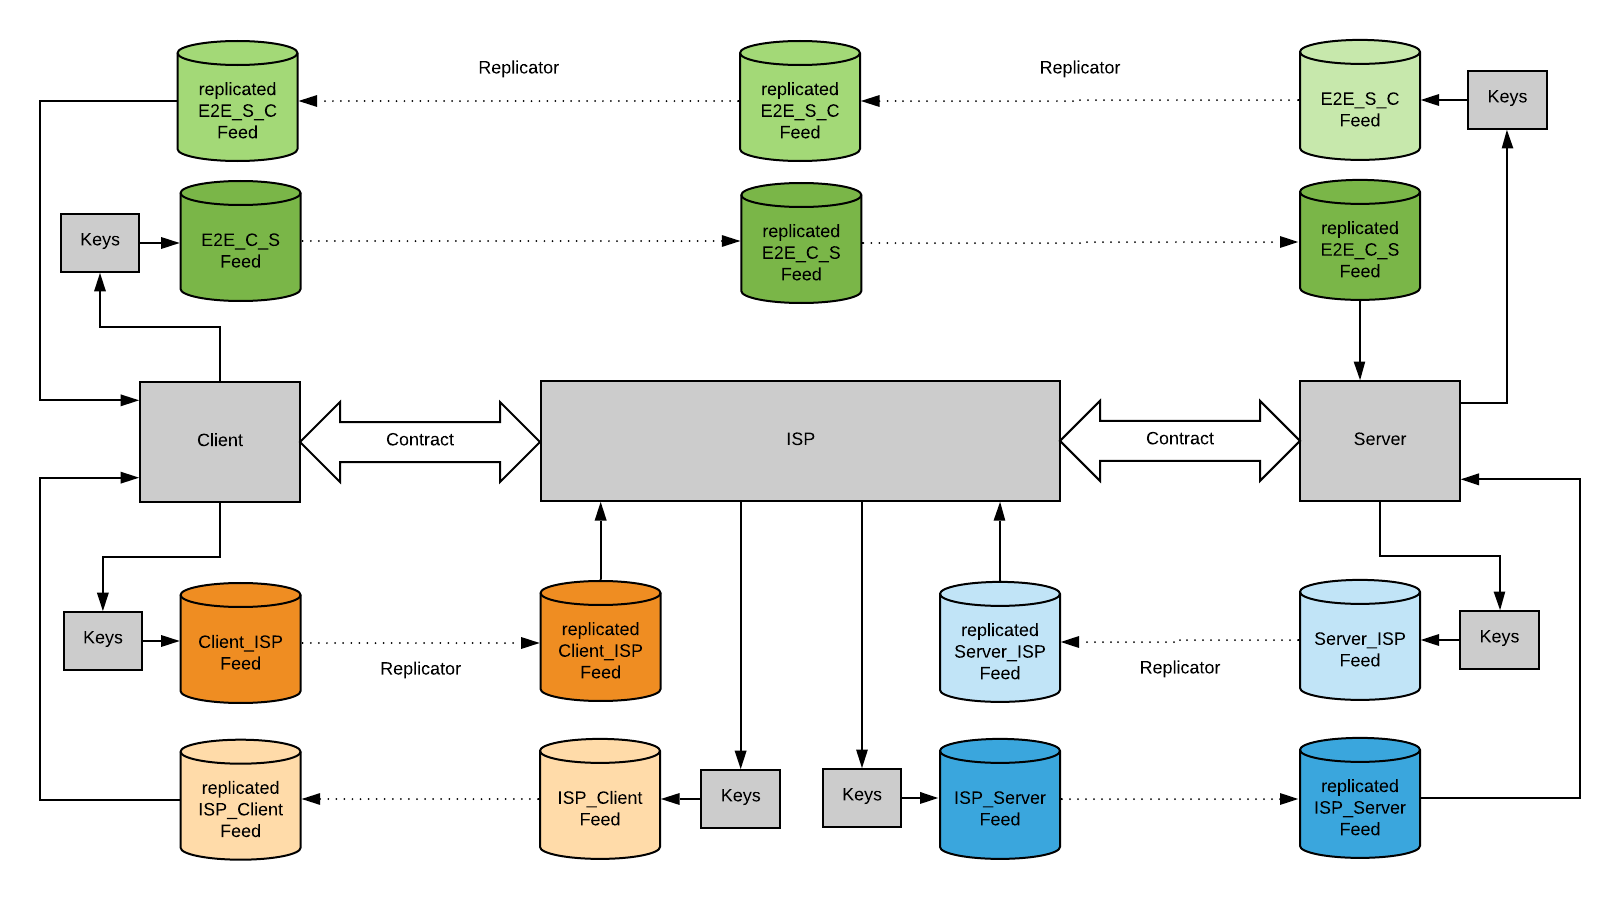
\includegraphics[width=0.9\textwidth]{intro_detru}
    \caption{State after accepted introduce from cli001 to ser001}
    \label{fig:contract_cli_isp}
\end{figure}

\pagebreak

%\section{0.4}
%added indirect communication from client to server over ISP\\
\section{Bundling}
taking again a look at the real world problem the isp has arbitrary many clients and many of them want to cumminicate with the same server. Idea: bundling all e2e feeds to same server into isp-server feed.
-> load on wire problem

\subsection{Adapted Introducing and Detrucing}
introducing to server same - after server accept server generates both feeds request and result feed - sends contract to isp and isp generates result feed and replicates to cli - finally client generates request feed and replicates to isp.


\subsection{Multiplexing and Demultiplexing}
requests from client same way to isp. but isp does not replicate feed anymore. it takes whole log entry, signed by client and mulutiplexes into a new log entry with a mux type content and signs this - mutliplexing. at server, server takes this mux type and extracts whole request feed entry and appends bytes to request feed from client - demultiplexing. handles request and writes result to result feed. from there the whole entry gets again multiplexed in the ispser feed. at isp isp demux entry and also appends bytewise to result feed. replicates to cli and cli can use result.

Resulting Schema:

\begin{figure}
    \centering
    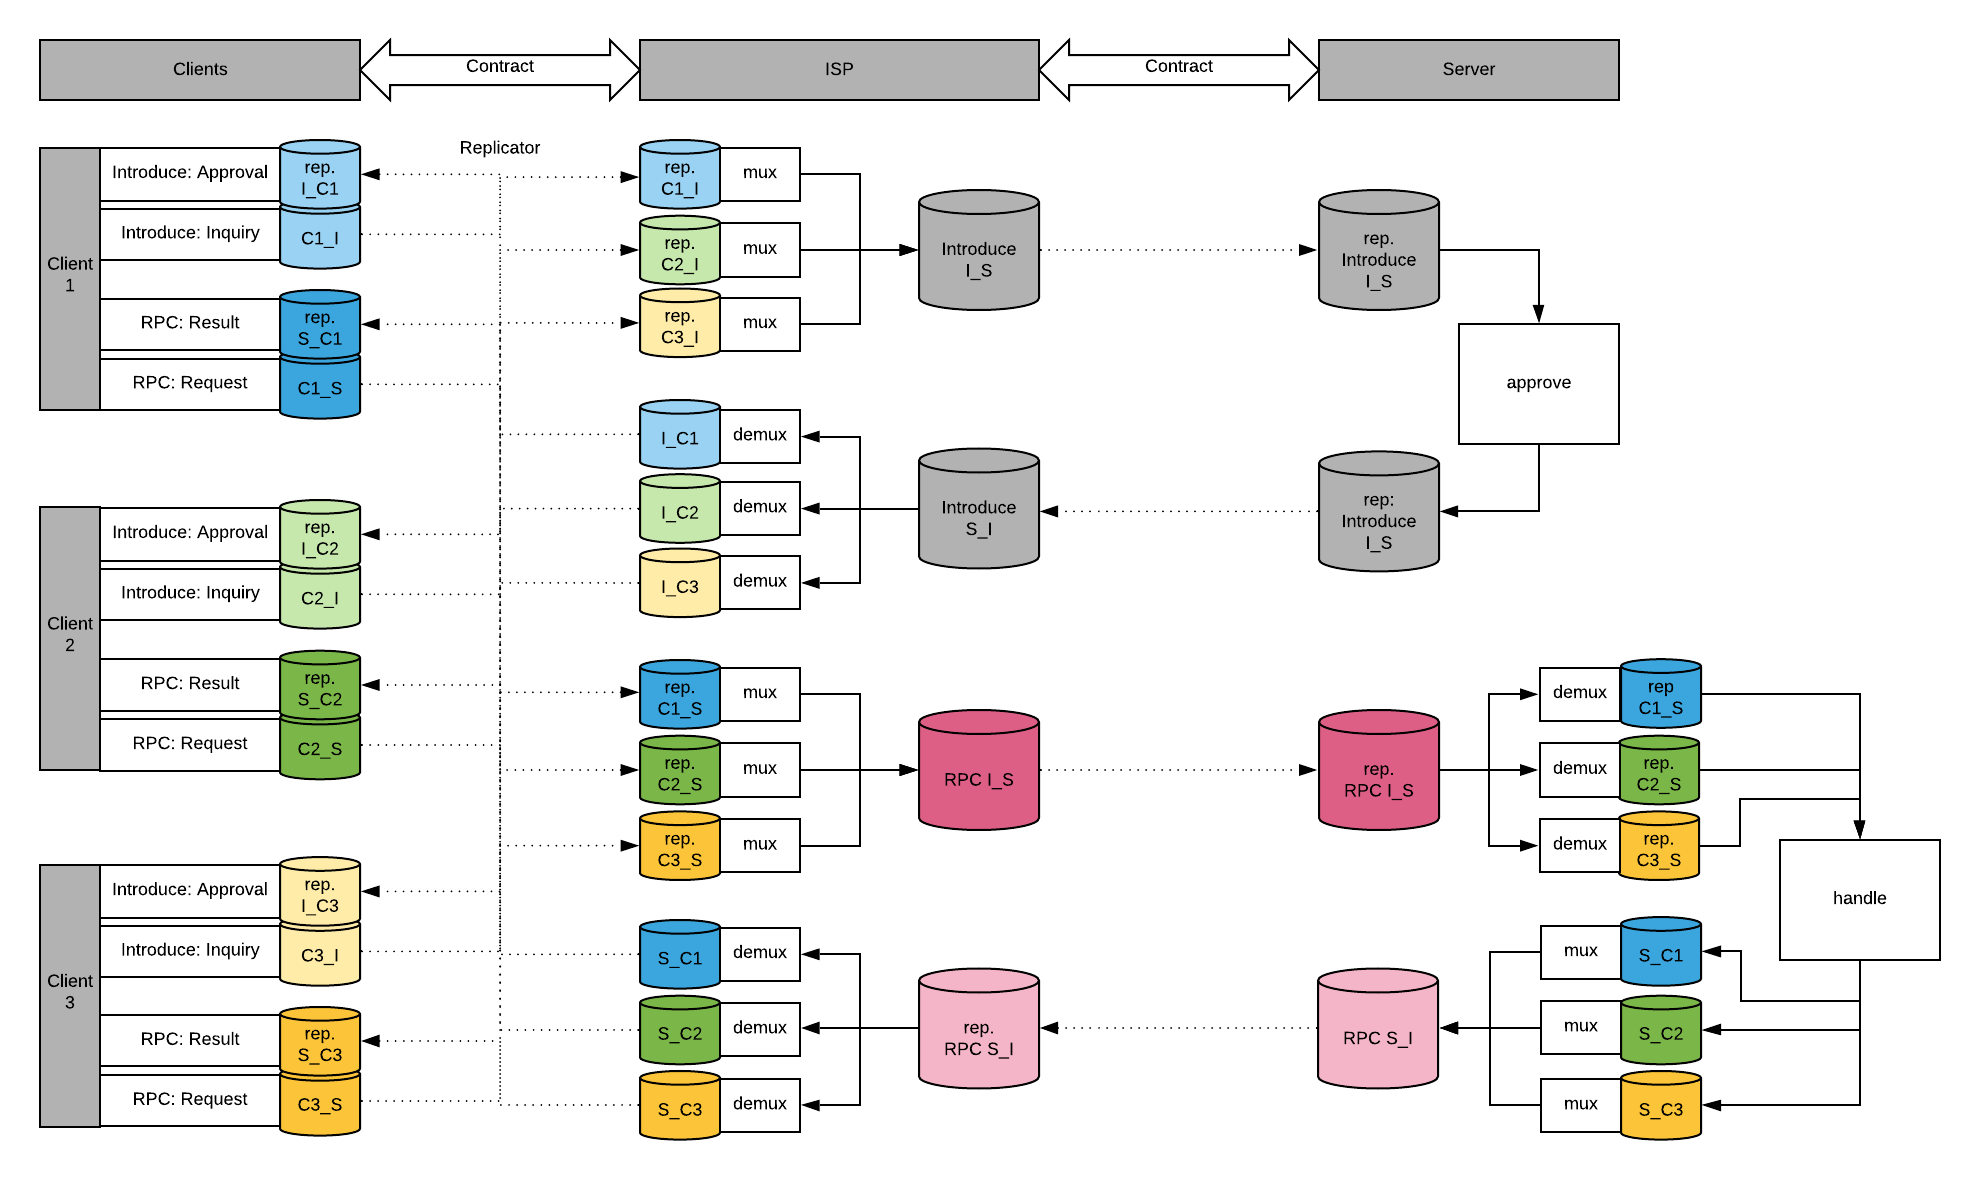
\includegraphics[width=0.9\textwidth]{mux_schema}
    \caption{multiplexing}
    \label{fig:mux}
\end{figure}

\section{Outlook}
\subsection{P2P ISP Nodes}
\subsection{Contract between ISPs}